% $HeadURL$

\subsection{Glyph: \glyph{Clone Marker}}
\label{sec:cloneMarker}

If an EPN is duplicated on a map, it is necessary to indicate this fact by using the \glyph{clone marker} auxiliary unit.  The purpose of this marker is to provide the reader with a visual indication that this node has been cloned, and that at least one other occurrence of the EPN can be found in the map (or in a submap; see \sect{submap}).  The clone marker takes two forms, simple and labeled, depending on whether the node being cloned can carry state variables (\ie whether it is a stateful EPN).


\subsubsection{Simple Clone Marker}

As mentioned above, the \glyph{simple clone marker} is the unlabeled version of the \glyph{clone marker}.  See below for the labeled version.


\begin{glyphDescription}

\glyphSboTerm Not applicable.

\glyphContainer The simple (unlabeled) \glyph{clone marker} is a portion of the surface of an EPN that has been modified visually through the use of a different shade, texture, or color.  \fig{simpleCloneMarker} illustrates this.  The \glyph{clone marker} occupies the lower part of the EPN glyph and the marker's surface must not exceed 30\% of the EPN's surface.

\glyphLabel Not applicable.

\glyphAux A \glyph{clone marker} does not carry any auxiliary items.

\end{glyphDescription}

\begin{figure}[H]
  \centering
  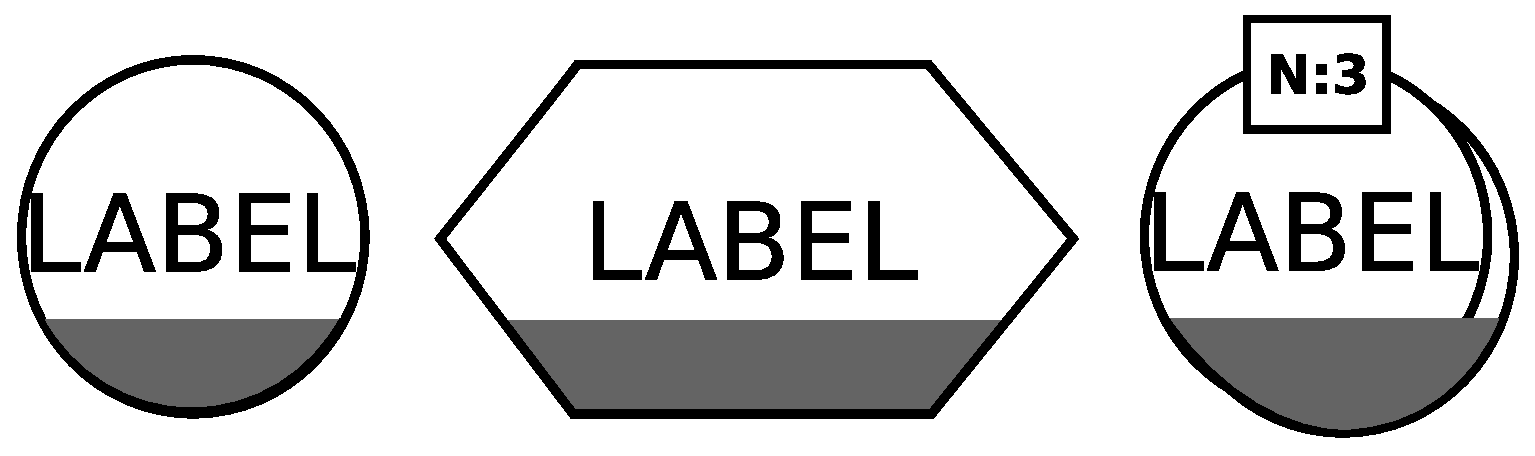
\includegraphics[scale = 0.3]{images/simpleCloneMarker}
  \caption{The \PD glyph for \glyph{clone marker}.}
  \label{fig:simpleCloneMarker}
\end{figure}


\subsubsection{Labeled Clone Marker}

Unlike the \glyph{simple clone marker}, the \glyph{labeled clone marker} includes (unsurprisingly, given its name) an identifying label that can be used to identify equivalent clones elsewhere in the diagram.  This is particularly useful for stateful EPNs, because these can have a large number of state variables displayed and therefore may be difficult to visually identify as being identical.

\begin{glyphDescription}

\glyphSboTerm Not applicable.

\glyphContainer The labeled \glyph{clone marker} is a portion of the surface of an EPN that has been modified visually through the use of a different shade, texture, or color.  The \glyph{clone marker} occupies the lower part of the EPN glyph the marker's surface must not exceed 30\% of the EPN's surface.

\glyphLabel A \glyph{clone marker} is identified by a label placed in an unbordered box containing a string of characters.  The characters can be distributed on several lines to improve readability, although this is not mandatory.  The label box must be attached to the center of the container.  The label may spill outside of the container.  The font color of the label and the color of the clone marker should contrast with one another.  The label on a labeled \glyph{labeled clone marker} is mandatory.

\glyphAux A \glyph{clone marker} does not carry any auxiliary items.

\end{glyphDescription}

\begin{figure}[H]
  \centering
  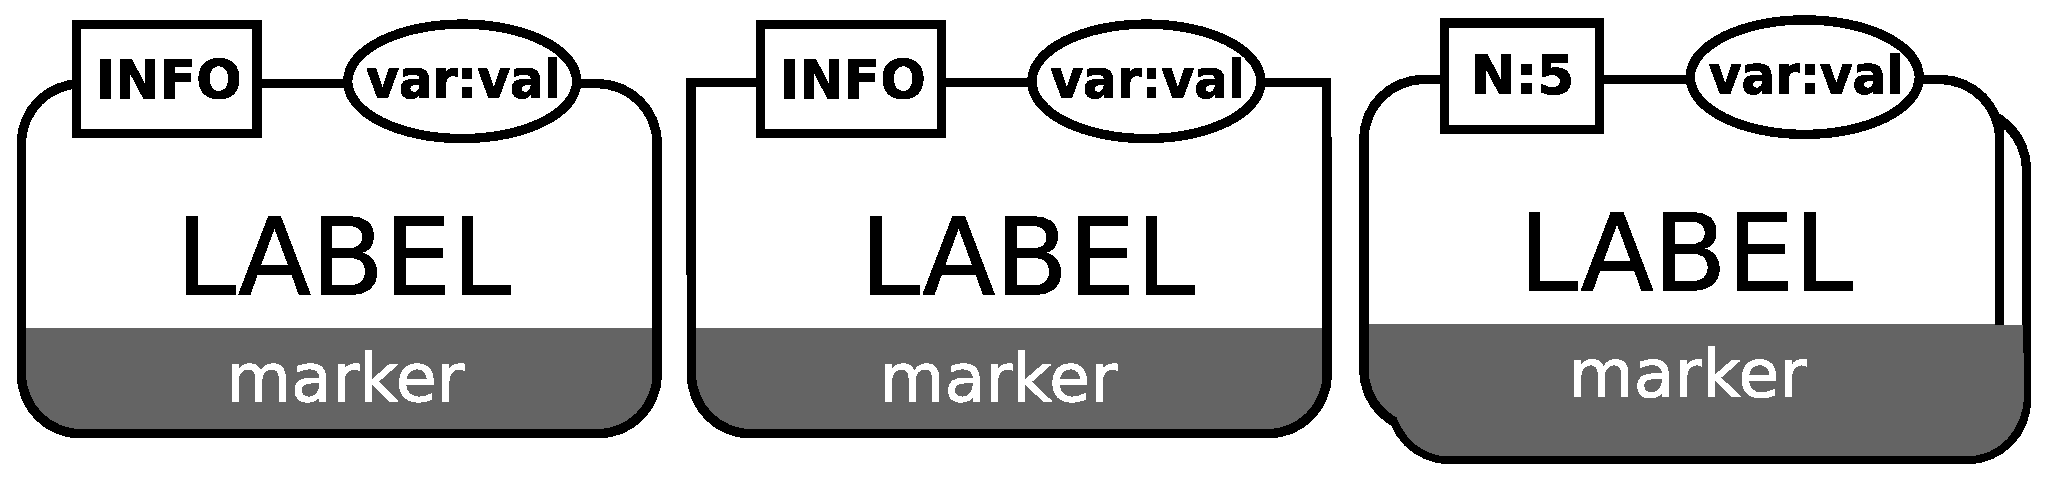
\includegraphics[scale = 0.3]{images/labeledCloneMarker}
  \caption{The \PD glyph for \glyph{labeled clone marker}.}
  \label{fig:labeledCloneMarker}
\end{figure}

\fig{example-cloning} contains an example in which we illustrate the use of \glyph{clone markers} to clone the species ATP and ADP participating in different reactions.  This example also demonstrates the chief drawbacks of using clones: it leads to a kind of dissociation of the overall network and multiplies the number of nodes required, requiring more work on the part of the reader to interpret the result.  Sometimes these disadvantages are offset in larger diagrams by a reduction in the overall number of line crossings, but not always.  In general, we advise that cloning should be used sparingly.

\begin{figure}[H]
  \centering
  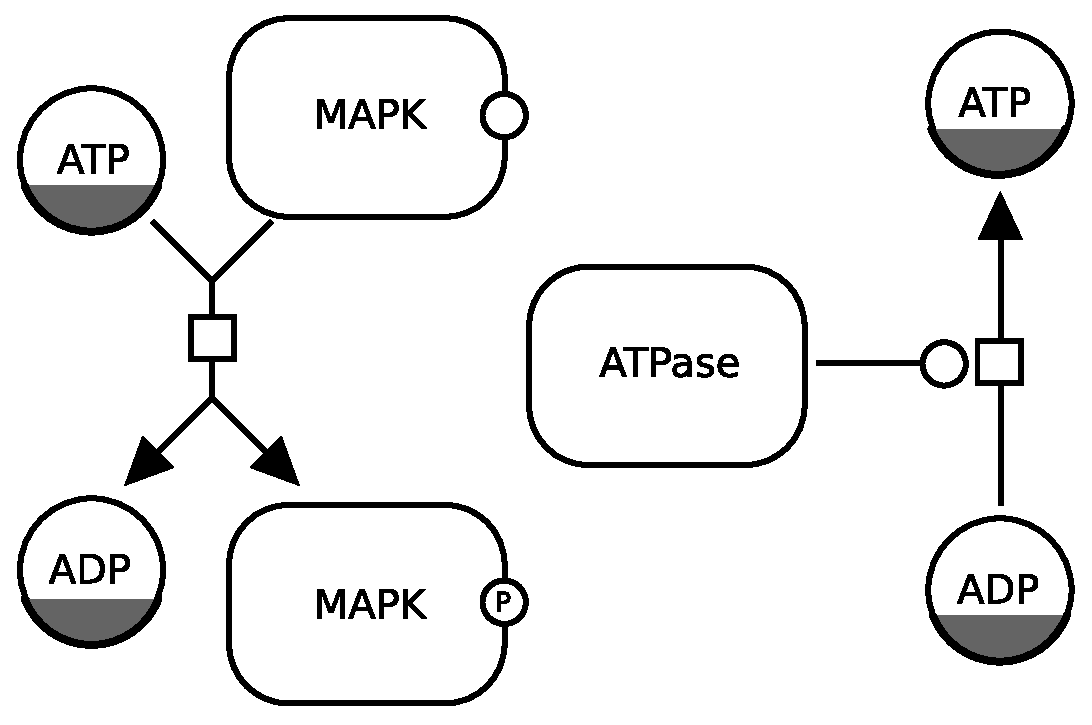
\includegraphics[scale = 0.5]{examples/cloning}
  \caption{An example of using cloning, here for the species ATP and ADP.}
  \label{fig:example-cloning}
\end{figure}




% The following is for [X]Emacs users.  Please leave in place.
% Local Variables:
% TeX-master: "../sbgn_PD-level1"
% End:
